\documentclass{beamer}

\usepackage[utf8]{inputenc}
\usepackage{tikz}
\usepackage{amssymb}
\usepackage{minted}
\usepackage{natbib}
\usepackage{pdfpages}
\usepackage{listings}
\usepackage{stmaryrd}

\setbeamertemplate{itemize items}[square]

\begin{document}
\title{Rebooting Supercompilation for Haskell}

\author[Ömer\,S.\,Ağacan \& Ryan\,R.\,Newton]
{%
  \texorpdfstring{
    \begin{columns}
      \column{.45\linewidth}
      \centering
      Ömer S. Ağacan\\
      \href{mailto:oagacan@indiana.edu}{oagacan@indiana.edu}
      \column{.45\linewidth}
      \centering
      Ryan R. Newton\\
      \href{mailto:rrnewton@indiana.edu}{rrnewton@indiana.edu}
    \end{columns}
  }
  {Ömer\,S.\,Ağacan \& Ryan\,R.\,Newton}
}

\date{\today}

\frame{\titlepage}

%\frame{\frametitle{Table of contents}\tableofcontents}

\begin{frame}
    \frametitle{Rebooting Supercompilation for Haskell - Talk outline}

    \begin{itemize}[<+->]
        \item
            An overview of supercompilation.
        \item
            What's interesting about it in the context of Haskell? Current
            state-of-the-art.
        \item
            Overview of how it works.
        \item
            "But where's my supercompiler for Haskell?" My preliminary work and
            research goals.
    \end{itemize}
\end{frame}

\begin{frame}[fragile]

    \frametitle{Supercompilation: An overview}

    \begin{itemize}[<+->]
        \item
            The paper that describes the idea in English: "The Concept of a
            Supercompiler" \citet{Turchin86theconcept}.
        \item
            High-level idea:
            \setbeamertemplate{itemize items}[circle]
            \begin{itemize}
                \item
                    Evaluate programs in compile-time, while making the most out
                    of known inputs and definitions.
                    \setbeamertemplate{itemize items}[square]
                    \begin{itemize}[]
                        \item
                            When evaluating sub-expressions of a case
                            expression, propagate information about current
                            branch(shape of the scrutinee).
                            \begin{lstlisting}[mathescape]
case v of
  P $v_1$ .. $v_N$  $\rightarrow$ expr
                            \end{lstlisting}

                            Evaluate $expr [ P\, v_1\, ..\, v_N \slash v ]$.
                    \end{itemize}
                \item
                    Most of the time the goal is to generate more efficient
                    programs. (but see \citet{Klyuchnikov2010proving} for a
                    different use of supercompilation)
            \end{itemize}
    \end{itemize}

\end{frame}

\begin{frame}
    \frametitle{Supercompilation in the context of Haskell}

    \begin{itemize}
        \item
            Why is it interesting?
        \item
            In a sense, it's the "ultimate" optimization. ("-O99")
        \item
            This optimizes in the sense that:

            If we have a programs $\mathcal{P}_1$ and $\mathcal{P}_2$, and
            \newline
            $\mathcal{P}_1 \Downarrow v$ in $N$ steps and \newline
            $\mathcal{P}_2 \Downarrow v$ in $M$ steps, \newline
            we consider $\mathcal{P}_2$ optimized if $M \textless N$.
        \item
            An approximation, but works well in practice.
            \newline
            (i.e. if $M \textless N$ then usually $M$ is a faster program)
    \end{itemize}
\end{frame}


\begin{frame}
    \frametitle{Supercompilation in the context of Haskell}

    \begin{itemize}
        \item[]
            It generalizes:
            \begin{itemize}
                \item
                    Deforestation(\citet{deforestation})
                \item
                    Partial evaluation
                \item
                    Call-pattern specialization(\citet{callpatternspec})
                \item
                    Ad-hoc optimizations via rewrite rules, e.g. shortcut fusion
                    (\citet{shortcutdeforestation}) or library-specific rewrite
                    rules
                \item
                    "Optimizing SYB is Easy!"(\citet{optimizingsyb}) and
                    "Optimizing Generics is Easy!"(\citet{optimizinggenerics})
                    style "domain-specific" partial evaluators
                \item
                    Function specialization(\texttt{SPECIALIZE} pragmas)
                \item
                    ... and many more
            \end{itemize}
    \end{itemize}
\end{frame}

\begin{frame}
    \frametitle{Current state-of-the-art}

    \begin{itemize}
        \item
            \citet{callbyneed-sc} shows some great potential:
            \begin{itemize}
                \item
                    Up to $20x$ faster runtime.
                \item
                    Up to $100\%$ reduction in allocation.
            \end{itemize}
        \item
            But it also suffers from problems that are inherent to
            supercompilation:
            \begin{itemize}
                \item
                    "We do not attempt to supercompile the full Nofib suite because the
                    other Nofib benchmarks are considerably more complicated and
                    generally suffer from extremely long supercompilation times."
                    \newline
                    (\citet{timeandspace} focuses on compilation performance,
                    and reports \textit{$<$3 seconds} for all the small programs
                    from Nofib)
                \item
                    Up to $132x$ compile time.
                \item
                    Up to $2.8x$ generated code size.
            \end{itemize}
    \end{itemize}
\end{frame}

\begin{frame}
    \frametitle{How it works? An overview}

    \begin{itemize}
        \item[]
            \citet{callbyneed-sc} laid out a great framework for
            supercompiling Haskell:
            \begin{itemize}[<+->]
                \item
                    \textcolor{blue}{Driving:} Take steps according to operational
                    semantics.  Some additional steps like case-of-case
                    transformation(\citet{Jones98atransformation-based}).
                \item
                    \textcolor{blue}{Splitting:} When stuck, keep evaluating
                    sub-expressions. Propagate information. After evaluating
                    sub-expressions combine results.
                \item
                    \textcolor{blue}{Matching:} Evaluating open terms lead to loops.
                    Matcher tries to detect loops, returns information about how
                    to refer to this new loop.
                \item
                    \textcolor{blue}{Termination checking:} Because perfect matcher is
                    not possible, and some programs just loop.
            \end{itemize}
    \end{itemize}
\end{frame}

{
    \setbeamercolor{background canvas}{bg=}
    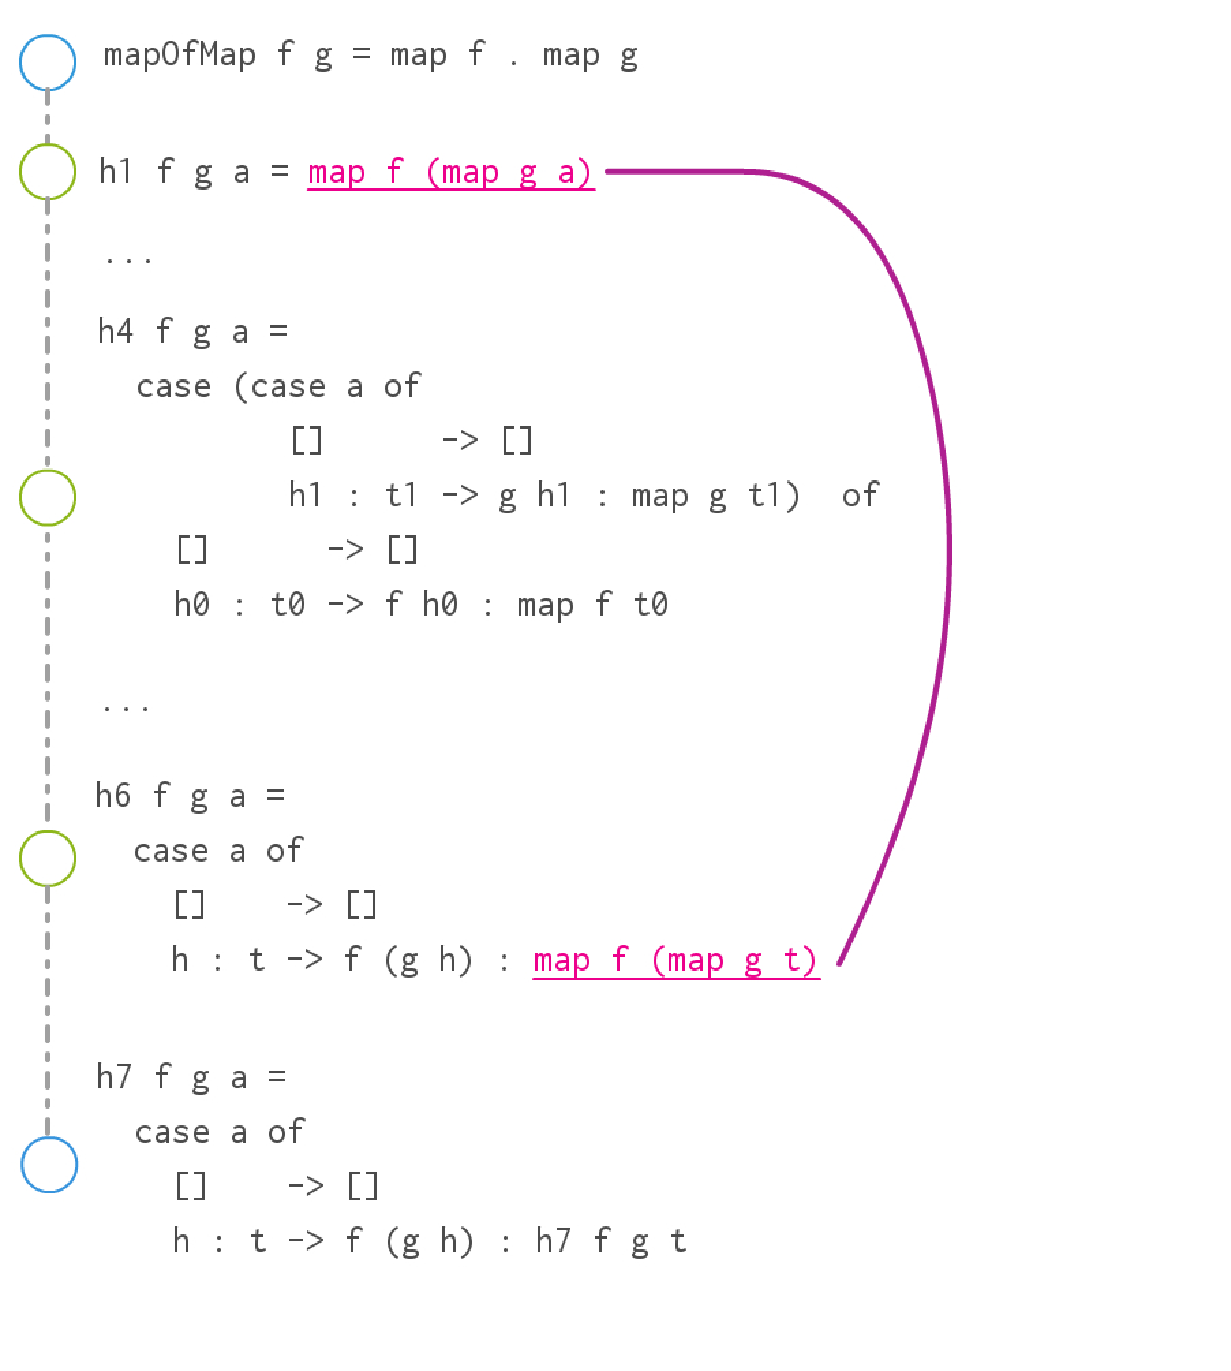
\includepdf[pages={1}]{mapOfMap.pdf}
}

\begin{frame}[fragile]
    \frametitle{Problems with supercompilation operations}

    \begin{itemize}[<+->]
        \item[]
            Each operation has hard problems to solve.

        \item[]
            \textcolor{blue}{Splitter:}
            (from \citet{callbyneed-sc})
            \begin{itemize}
                \item[]
                    Propagating too much information may lead to work
                    duplication.

                    \begin{minted}{haskell}
let n = fib 100
    b = n + 1
    c = n + 2
 in (b, c)
                    \end{minted}

                \item[]
                    Propagating too little information may lead to missing
                    optimization opportunities.
                    \begin{minted}{haskell}
let map = . . .
    ys = map f zs
    xs = map g ys
 in Just xs
                    \end{minted}
            \end{itemize}
    \end{itemize}
\end{frame}

\begin{frame}[fragile]
    \frametitle{Problems with supercompilation operations}

    \begin{itemize}[<+->]
        \item[]
            Each operation has hard problems to solve.

        \item[]
            \textcolor{blue}{Matcher:}
            \begin{itemize}
                \item[]
                    May lead to work sharing, which may increase memory
                    residency. (\citet{commonsubexpression})

                    \begin{minted}{haskell}
S0 =
    let a = fib y
        b = fib y
     in (a, b)

S1 =
    let a = fib y
     in (a, a)
                    \end{minted}

                \item[]
                    Or:

                \item[]
                    \begin{minted}{haskell}
S0 = sum [1 .. 1000] + prod [1 .. 1000]
S1 = let l = [1 .. 1000] in sum l + prod l
                    \end{minted}

            \end{itemize}
    \end{itemize}
\end{frame}

\begin{frame}[fragile]
    \frametitle{Problems with supercompilation operations}

    \begin{itemize}[<+->]

        \item[]
            Each operation has hard problems to solve.

        \item[]
            \textcolor{blue}{Termination checker:}

            \begin{itemize}

                \item[]
                    Some programs just loop.

                    \begin{minted}{haskell}
loop n = loop (n + 1)
countFrom n = n : countFrom (n + 1)
                    \end{minted}

                \item[]
                    Sometimes detecting loops is not so easy: (growing
                    arguments)

                    \begin{minted}{haskell}
reverse_acc []      acc = acc
reverse_acc (h : t) acc = reverse_acc t (h : acc)
goal lst = reverse_acc (reverse_acc lst []) []
...
h_ lst = ... reverse_acc t1 (h1 : []) ...
...
h_ lst = ... reverse_acc t2 (h2 : h1 : []) ...
...
                    \end{minted}

            \end{itemize}

    \end{itemize}
\end{frame}

\begin{frame}
    \frametitle{"Where's my supercompiler for Haskell?"}

    \begin{itemize}[<+->]
        \item
            \citet{callbyneed-sc} has some solutions, and it documents and
            implements it nicely.

        \item
            But we still don't have something that we can use \textit{today.}

        \item
            I'm rebooting the supercompiler!

        \item
            The goal here is to distribute it as a package, downloadable from
            Hackage.

        \item
            Then the research will follow.
    \end{itemize}
\end{frame}

\begin{frame}
    \frametitle{Current status and problems}

    \begin{itemize}
        \item[]
            There has been some changes in GHC:

            \begin{itemize}
                \item
                    Some changes in the Core theory: Roles.
                \item
                    Lots of refactoring.
            \end{itemize}

        \item[]
            GHC API related problems:

            \begin{itemize}
                \item
                    Some needed internals are not exposed by GHC -- requires
                    some modifications in GHC.
                \item
                    No easy ways to do most basic stuff: Moving terms
                    around(substitutions), known-case reduction, case-of-case,
                    etc.  (all done in some parts of Core-to-Core passes, need
                    to reverse engineer)
                \item
                    No easy way to annotate Core syntax. Duplicating the syntax
                    means duplicating huge amounts of code.
                \item
                    Working on Core is hard: Invariants are encoded as partial
                    functions without any helpful error messages -- if we're
                    lucky, there's a NOTE.
                \item
                    Some things are not clear. (Types are first-class, but can I
                    use them wherever I want? The Core definition allows this)
            \end{itemize}

    \end{itemize}
\end{frame}

\begin{frame}
    \frametitle{Conclusions}

    \begin{itemize}[<+->]
        \item[]
            Have a working implementation of supercompiler described in
            \citet{callbyneed-sc}.
        \item[]
            (Maybe) Improve GHC plugin API on the way.
        \item[]
            Collecting benchmark programs - send yours! (with expected
            optimizations)
            \newline
            We can create a benchmark suite like Nofib, but for
            supercompilation-specific problems. (pathological cases, programs
            with lots of intermediate data structures)
    \end{itemize}
\end{frame}

\begin{frame}
    Once we have a working implementation:
    \begin{itemize}
        \item
            Focus on specific parts(matcher, splitter etc.). Try other
            ideas from the literature(e.g. homeomorphic embedding).
        \item
            Work on some of the obvious improvements, like parallelizing
            the matcher.
        \item
            More experimental ideas:
            \begin{itemize}
                \item[]
                    Can we formulate it as a search problem and apply
                    ideas from the literature?
                \item[]
                    Are profile-driven decision making possible?
                \item[]
                    Are machine learning algorithms applicable?
            \end{itemize}
    \end{itemize}
\end{frame}

\begin{frame}
    Once we have a working implementation:
    \begin{itemize}
        \item
            Focus on specific parts(matcher, splitter etc.). Try other
            ideas from the literature(e.g. homeomorphic embedding).
        \item
            Work on some of the obvious improvements, like parallelizing
            the matcher.
        \item
            More experimental ideas:
            \begin{itemize}
                \item[]
                    Can we formulate it as a search problem and apply
                    ideas from the literature?
                \item[]
                    Are profile-driven decision making possible?
                \item[]
                    Are machine learning algorithms applicable?
            \end{itemize}
    \end{itemize}

    \bigskip
    Thanks!
    \newline
    Github: osa1/sc-plugin \hspace{0.3cm} IRC: osa1 \hspace{0.3cm} Mail:
    oagacan@indiana.edu

\end{frame}

\begin{frame}[allowframebreaks]
    \frametitle{References}

    \bibliographystyle{abbrvnat}
    \bibliography{refs}
\end{frame}

\end{document}
